%! TeX program = lualatex
\documentclass[../main.tex]{subfiles}
\begin{document} 

\centerline{\includegraphics[width=\pagewidth]{../standalones/image-toucan}}

{\footnotesize Image credit: \href{https://www.flickr.com/photos/8070463@N03/9324653982}{``Toucan from the other side'' by Tambako the Jaguar} is licensed under CC BY-ND 2.0.}

\section{A toucan of truth?}
\begin{example} \label{ex:toucan}
  In this example, work in small teams to evaluate scientific arguments. Carefully read through the four parts of this activity: \emph{the setup}, \emph{the data}, \emph{the question} and \emph{the arguments}. Finally, discuss within your group which intern's argument you choose to accept.

  \begin{enumerate}[wide, label=(\arabic*)]
    \item \emph{The setup}. An ecologist visits Costa Rica to study birds. They bring back data \hlmain{relating sizes of birds and their weights}. 
      Sizes of birds are challenging to quantify due to their complex geometries, so the ecologist makes a \hlsupp{simplification} and treats birds as if they were perfect cubes. We define the \hlmain{length} \(\ell\) of a bird to be the side length of the smallest perfect cube containing the bird.

      \begin{figure}[H]
        \centering
        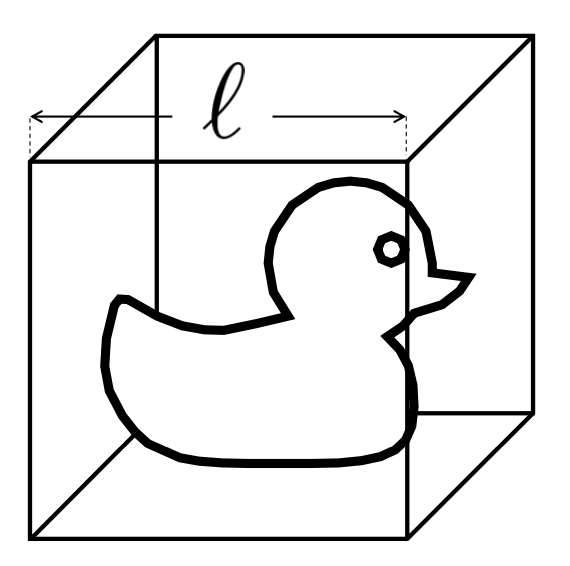
\includegraphics[width=2in]{../standalones/image-bird-cube.png}
      \end{figure}

    \item \emph{The data}. Explore the ecologist's data on the following plots.

      \centerline{
        \includegraphics{../standalones/build/plot-birds-of-costa-rica}
        \includegraphics{../standalones/build/plot-birds-of-costa-rica-loglog}
        \includegraphics{../standalones/build/plot-birds-of-costa-rica-loglog-zoomed-in}
      }

    \item \emph{The question}. The ecologist does not have data on toucans and is \emph{interested} in this question:
      \begin{center}
        \hlmain{How much does an adult toucan weigh given that its length is roughly 40 cm?}
      \end{center}

    \item \emph{The arguments}. Two interns put forth their analysis. 
      \begin{enumerate}[wide, label=Intern \Alph*:]
        \item A cubic model \(w = 0.006 \ell^{3}\) fits the data.
        \item A quadratic model \(w = 0.25 \ell^{2}\) also fits the data.
      \end{enumerate}

      \includegraphics{../standalones/build/plot-birds-of-costa-rica-arg1}
      \includegraphics{../standalones/build/plot-birds-of-costa-rica-arg2}
  \end{enumerate}

  \medskip
  \begin{mdframed}[roundcorner=10pt]
    \textbf{Your turn!} Interestingly, both arguments lead to \emph{remarkably similar} predictions that an adult toucan should weight about \(400\) grams.
    \begin{center}
      \hlmain{\faComment{} \large You are the ecologist. How do you evaluate your interns' arguments?}
    \end{center}

    \hlsupp{Apply dimensional homogeneity and log-log transformation to support your arguments.}
  \end{mdframed}

  Articulate your thoughts and record any associated calculations on the next page.

  \blanklines{50}
\end{example}
\end{document}
